\section{Patterns: Design and Implementation}
\label{section:patterns}

In this section, we will introduce the \emph{patterns} which form the expressions written by the programmer and used for code generation.
As we saw in the previous section there exist two type of patterns: high-level algorithmic patterns and low-level \OpenCL patterns.
Some of the high-level algorithmic patterns directly correspond to algorithmic skeletons we have introduced in \autoref{chapter:skelcl}.
As we will also introduce patterns which we have not seen so far and which do not oblige to the common definition of algorithmic skeletons, we will use the more generic term \emph{pattern} throughout this and the next chapter.

The key idea of our approach is to expose algorithmic choices and hardware-specific program optimizations as rewrite rules (discussed later in \autoref{section:rules}) which systematically transform pattern-based expressions.
The high-level algorithmic patterns represent structured parallelism.
They can either be used by the programmer directly as a stand-alone language, but could also be used as a domain specific language embedded in a general purpose programming language, or used as an intermediate representation targeted by the compiler of another programming language.
Once a program is represented with our high-level patterns, we systematically transform the program into low-level patterns.
The low-level patterns represent hardware-specific concepts expressed by a programming model such as \OpenCL, which is the target chosen for this thesis.
Following the same methodology, a different set of low-level patterns could be designed to target other low-level programming models such as Pthreads or \MPI.


\subsection{High-level Algorithmic Patterns}

We define our patterns as functions.
To simplify our implementation, we encode all types as arrays with primitives represented by arrays of length 1.
The only exceptions are the user-defined functions, such as the \code{mul3} function in \autoref{fig:codeex:map} that operates on primitive types.

\autoref{tab:hlskel} presents our high-level patterns used to define programs at the algorithmic level.
Most of the patterns are well known in functional programming, like \map and \reduce.
The \zip, \splitN and \join patterns transform the shape of the data.
The \iterateN pattern iteratively applies a function multiple times.
Finally, the \reorder pattern lets our system know that it is safe to reorder the elements of an array arbitrarily, which enables additional optimizations -- as we will see later in \autoref{chapter:codeGeneration-evaluation}.

In the following, we discuss each high-level algorithmic pattern in more detail including their formal definitions.
As in \autoref{chapter:skelcl} we use the Bird-Meertens formalism~\cite{Bird88} as inspiration for our notation of the patterns.
For full details on the notation see~\autoref{par:notation} on page~\pageref{par:notation}.
Here is a short reminder of our notation:
we write function application using a space and functions are often curried;
binary operators (\eg, $\oplus$) are written using infix notation and can be written using prefix notation when being sectioned by using parenthesis, \ie,:
$a\ \oplus\ b = (\oplus)\ a\ b$.
For an array $xs$ of length $n$ with elements $x_i$ we write $[x_1, \ldots, x_n]$.

In this chapter we are especially interested in how patterns can be composed and nested.
As \emph{types} formally specify which compositions and nesting of patterns are legal, we will define the type of each pattern.
% For expressing types we base our syntax on the syntax established by J. Roger Hindley, Robin Miler, and Luis Damas as part of the Hindley---Milner type system~\cite{}.
We write $e : \sigma$ to denote that expression $e$ has type $\sigma$.
% To make typing judgments we write $e_0 : \sigma_0,\ \ldots,\ e_n : \sigma_n\ \vdash e : \sigma$ to denote that under the assumptions that $e_0,\ \ldots,\ e_n$ have types $\sigma_0,\ \ldots,\ \sigma_n$ the expression $e$ has type $\sigma$.
For a function mapping values of type $\alpha$ to values of type $\beta$ we write its type as $(\alpha \rightarrow \beta)$.
Tuple types are written as $\langle\alpha, \beta\rangle$.
Finally, arrays have their length denoted as part of their type:
for an array with elements of type $\alpha$ and length $n$, we write $[\alpha]_n$.

A formal description of a core subset of the patterns described in this section can also be found in our paper~\cite{SteuwerFeLiDu2015}, where formal syntax, typing rules, and formal semantics using a denotational style are given.

\begin{table}[t]
\centering
\begin{tabular}{p{.125\textwidth}p{.75\textwidth}}
\toprule
\tabhead{Pattern} & \tabhead{Description}\\
\midrule
 \map
     & Apply a given function to every element of an input array.\\
 \reduce
     & Perform a reduction of an input array using a user-defined binary function and an initial value.\\
 \zip
     & Build an array of pairs by pairwise combining two arrays.\\
 \splitN
     & Produce a multi-dimensional array by splitting an array in chunks of a given size.\\
 \join
     & Join the two outer most dimensions of an multi-dimensional array.\\
 \iterateN
     & Iterate a given function over an input array a fixed number of times.\\
 \reorder
     & Reorder the element of the input array.\\
\bottomrule
\end{tabular}
\caption{High-level algorithmic patterns used by the programmer.}
\label{tab:hlskel}
\end{table}


\paragraph{Map}
The \map pattern is well known in functional programming and applies a given unary function $f$ to all elements of an input array.
In \autoref{chapter:skelcl}, we defined the \map pattern as an algorithmic skeleton (see \autoref{definition:map}).
The same definition holds here.
We repeat it here for completeness and we add the type information:
\begin{definition}
  \label{definition:pattern:map}
  Let $xs$ be an array of size $n$ with elements $x_i$ where $0 < i \leq n$.
  Let $f$ be a unary customizing function defined on elements.
  The \map pattern is then defined as follows:
  \begin{equation*}
    \map\ f\ [x_1, x_2, \dots, x_n] \eqdef [f\ x_1, f\ x_2, \dots, f\ x_n]
  \end{equation*}
  The types of $f$, $xs$, and \map are as follows:
  \begin{align*}
    f &: (\alpha \rightarrow \beta),\\
    xs &: [\alpha]_n,\\
    \map\ f\ xs &: [\beta]_n .
  \end{align*}
\end{definition}

\noindent
In \autoref{chapter:skelcl} we also defined the \map skeleton for operating on matrices (see \autoref{definition:map:matrix}).
In this chapter we represent matrices as nested arrays, therefore, performing an operation on each element of a matrix can be represented by nesting two \map patterns:
\begin{align*}
  mapMatrix\ \ f\ \ X &= \map\ (\map\ f)\ X
\end{align*}
Let us assume that $X$ represents an $n\times m$ matrix with elements of type $\alpha$, then its type is $\big[[\alpha]_m\big]_n$.
The outer \map applies its customizing function to every row of matrix $X$.
The customizing function is defined by currying \map and $f$, thus, producing a function which applies $f$ to every element of its argument array.
Therefore, $f$ will be applied to every element of matrix $X$.

\paragraph{Reduce}
The \reduce pattern (\aka, fold or accumulate) uses a binary operator $\oplus$ to combine all elements of the input array.
We require the operator $\oplus$ to be associative and commutative which allows for an efficient parallel implementation.
By requiring commutativity, our system can also generate vectorized implementations of the reduction and utilize the efficient coalesced memory access pattern.
These are crucial optimizations on modern \GPUs as we saw in \autoref{section:reduce:case-study}.
In \autoref{chapter:skelcl} we defined \reduce as an algorithmic skeleton (see \autoref{definition:reduce}).
The same definition holds here.
We repeat it here for completeness and we add the type information:
\begin{definition}
  \label{definition:pattern:reduce}
  Let $xs$ be an array of size $n$ with elements $x_i$ where $0 < i \leq n$.
  Let $\oplus$ be an associative and commutative binary customizing operator with the identity element $\id_\oplus$.
  The \reduce pattern is then defined as follows:
  \begin{equation*}
    \reduce\ (\oplus)\ \id_\oplus\ [x_1, x_2, \dots, x_n]
      \eqdef [x_1 \oplus x_2 \oplus \dots \oplus x_n]
  \end{equation*}
  The types of $(\oplus)$, $\id_\oplus$, $xs$, and \reduce are as follows:
  \begin{align*}
    (\oplus) &: ((\alpha, \alpha) \rightarrow \alpha),\\
    \id_\oplus &: \alpha,\\
    xs &: [\alpha]_n,\\
    \reduce\ (\oplus)\ \id_\oplus\ xs &: [\alpha]_1 .
  \end{align*}
\end{definition}

This definition is unambiguous and well-defined even without explicit parenthesis as we require the binary operator to be associative and commutative.

\paragraph{Zip}
The \zip pattern and the \splitN/\join patterns transform the shape of the data. %which we store in the type system, \ie, number of dimensions and size of each dimension.
The \zip pattern fuses two arrays into a single array of pairs.

\begin{definition}
  \label{definition:pattern:zip}
  Let $xs$ and $ys$ be arrays of size $n$ with elements $x_i$ and $y_i$ where $0 < i \leq n$.
  The \zip pattern is then defined as follows:
  \begin{equation*}
    \zip\ [x_1, x_2, \dots, x_n]\ [y_1, y_2, \dots, y_n]\\
      \eqdef [\langle x_1, y_1\rangle, \langle x_2, y_2\rangle, \dots, \langle x_n, y_n\rangle]
  \end{equation*}
  The types of $xs$, $ys$, and \zip are as follows:
  \begin{align*}
    xs &: [\alpha]_n,\\
    ys &: [\beta]_n,\\
    \zip\ xs\ ys &: [\langle\alpha, \beta\rangle]_n .
  \end{align*}
\end{definition}

\noindent
This definition significantly differs from the definition of the \zip skeleton in \autoref{chapter:skelcl}:
While in \autoref{definition:zip}, \zip applies a given function to pairs of elements, there is no function to be applied in \autoref{definition:pattern:zip} of the \zip pattern.
The behavior of the \zip skeleton from \SkelCL can be achieved by composing the \zip pattern with the \map pattern:
\begin{align*}
  zipWith\ f\ xs\ ys &= \map\ f\ (\zip\ xs\ ys)
\end{align*}


\paragraph{Split and Join}
The \splitN pattern, which is most often combined with the \join pattern, partitions an array into chunks of specific size, resulting in an extra dimension in the output array.

We start with the definition of the \splitN pattern.
\begin{definition}
  \label{definition:pattern:split}
  Let $n$ be an integer value.
  Let $xs$ be an array of size $m$ with elements $x_i$ where $0 < i \leq m$.
  Let us assume that $m$ is evenly divisible by $n$.
  The \splitN pattern is then defined as follows:
  \begin{align*}
    &\splitN\ n\ [x_1, x_2, \dots, x_m] \eqdef\\
    &\qquad\big[[x_1, \ldots, x_n], [x_{n+1}, \ldots, x_{2n}], \ldots, [x_{m-n+1}, \ldots, x_m]\big]
  \end{align*}
  The types of $n$, $xs$, and \splitN are as follows:
  \begin{align*}
    n &: int,\\
    xs &: [\alpha]_m,\\
    \splitN\ n\ xs &: \big[[\alpha]_n\big]_{\frac{m}{n}} .
  \end{align*}
\end{definition}

\bigskip
%The formal type of the \splitN pattern is:
%\begin{align}
%  n : int,\ xs : [\alpha]_m\ \vdash\ split\ n\ xs : \big[[\alpha]_n\big]_{{}^m/_n}
%\end{align}

\noindent
The corresponding \join pattern does the opposite:
it reassembles an array of arrays by merging dimensions.
\begin{definition}
  \label{definition:pattern:join}
  Let $xs$ be an array of size $\frac{m}{n}$ whose elements are arrays of size $n$.
  We denote the elements of the $i$th inner array as $x_{((i-1)\times n) + j}$ where $0 < i \leq \frac{m}{n}$ and $0 < j \leq n$.
  The \join pattern is then defined as follows:
  \begin{align*}
    &\join_n\ \big[[x_1, \ldots, x_n], [x_{n+1}, \ldots, x_{2n}], \ldots, [x_{m-n+1}, \ldots, x_m]\big] \eqdef\\
    &\qquad[x_1, x_2, \dots, x_m]
  \end{align*}
  The types of $xs$ and $\join_n$ are as follows:
  \begin{align*}
    xs &: \big[[\alpha]_n\big]_{\frac{m}{n}},\\
    \join_n\ xs &: [\alpha]_m .
  \end{align*}
\end{definition}

\noindent
We will almost always omit the subscript, as $n$ can be inferred from the length of the input array.
From these definitions it follows, that the compositions of \splitN and \join: $\join_n \circ \splitN\ n$ and $\splitN\ n \circ \join_n$ for any value $n$ yields the same type and also does not change any element in the array, \ie, it is equivalent to the identify function \emph{id}.

% These two patterns used together are similar to the split-join concept from data-flow languages such as StreamIt~\cite{ThiesKaAm2002}.


\paragraph{Iterate}
The \iterateN pattern corresponds to the mathematical definition of iteratively applying a function, which is defined as: {$f^0 = id$} and {$f^{n+1} = f^n \circ f$}.

\begin{definition}
  \label{definition:pattern:iterate}
  Let $n$ be an integer value with $n \geq 0$.
  Let $f$ be a unary function on arrays.
  Let $xs$ be an array of arbitrary size.
  We define the \iterateN pattern recursively:
  \begin{align*}
    \iterateN\ 0\ f\ xs &\eqdef xs,\\
    \iterateN\ n\ f\ xs &\eqdef \iterateN\ (n-1)\ f\ (f\ xs)
  \end{align*}
  The types of $n$, $f$, $xs$, and \iterateN are as follows:
  \begin{align*}
    n &: int,\\
    f &: ([\alpha]_k \rightarrow [\alpha]_{F(k)}),
      \begin{aligned}[t]
        & \forall k \text{ and where } \\
        &F : (int\rightarrow int) \text{ describes the change}\\
        &\text{of array length when applying } f,
      \end{aligned}\\
    xs &: [\alpha]_m,\\
    \iterateN\ n\ f\ xs &: [\alpha]_{F^n(m)} .
  \end{align*}
\end{definition}


% In terms of implementation, our code generator emits a for-loop to perform the iteration, and two pointers for input and output.
% After each iteration, we swap the pointers, so that the output of the last iteration becomes the input for the next one.
% We automatically allocated and calculate memory requirements based on the information from the input and output type.
\noindent
The type of the \iterateN pattern is interesting as its result type depends on the effect $f$ has on the size of its argument.
The index function $F$ describes the effect the function $f$ has on the length of its input array.
This index function is used to compute the effect the \iterateN function has when applying $f$ $n$ times on its input array.
Please note, that the length of the input array of $f$, \ie, $k$, possibly changes every time $f$ is applied by \iterateN.
% A more formal treatment of the topic can be found in our technical report~\cite{SteuwerFeLiDu2015}.
A formal treatment of the topic using a denotational semantics can be found in our paper~\cite{SteuwerFeLiDu2015}.

%\begin{align}
%  n : int,\ F : (int \rightarrow int),\ f : (\forall k\ .\ [\alpha]_k \rightarrow [\alpha]_{F(k)}),\ xs : [\alpha]_m\ %
%  \vdash iterate\ n\ f\ xs : [\alpha]_{F^{n}(m)}
%\end{align}

\paragraph{Reorder}
The \reorder pattern is used to specify that the ordering of the elements of an array does not matter.

\begin{definition}
  \label{definition:pattern:reorder}
  Let $xs$ be an array of size $n$ with elements $x_i$ where $0 < i \leq n$.
  Let $\sigma$ be an arbitrary permutation of $[1,\ldots, n]$.
  The \reorder pattern is then defined as follows:
  \begin{align*}
    \reorder\ [x_1, \ldots, x_n] &\eqdef [x_{\sigma(1)}, \ldots, x_{\sigma(n)}]
  \end{align*}
  The types of $xs$ and \reorder are as follows:
  \begin{align*}
    xs &: [\alpha]_n,\\
    \reorder\ xs &: [\alpha]_n
  \end{align*}
\end{definition}

\noindent
This definition allows to pick any permutation, \ie, a bijective function mapping values from the domain $[1,\ldots, n]$ to the image $[1,\ldots, n]$, for reordering the elements of an array arbitrarily which may enable optimizations, as we will see later.





\subsection{Low-level, \OpenCL-specific Patterns}

% Programming manycore CPU and GPU devices is difficult due to the need for managing parallelism, the memory hierarchy and other hardware specific features.
In order to achieve the highest performance, programmers often use a set of intuitive ``rules of thumb'' to optimize their applications.
We extensively discussed one application example in \autoref{section:reduce:case-study}.
Each hardware vendor provides own optimization guides~\cite{CUDAProgrammingGuide,AMDProgrammingGuide,IntelGPUProgrammingGuide,IntelXeonProgrammingGuide} that extensively cover vendor's hardware particularities and optimizations.
The main idea behind our approach is to identify common optimizations and express them systematically rather than intuitively, using low-level patterns coupled with a rewrite-rule system.

\autoref{tab:llskel} gives an overview of the \OpenCL-specific patterns we have identified.

\begin{table}[p]
\centering
\begin{tabular}{p{.225\textwidth}p{.7\textwidth}}
\toprule
\tabhead{Pattern} & \tabhead{Description}\\
\midrule
 \mapWorkgroup
     & Each \OpenCL \textbf{work-group} applies the given function to an element of the input array.\\
 \mapLocal
     & Each \textbf{local work-item} of a work-group applies the given function to an element of the input array.\\
 \mapGlobal
     & Each \textbf{global work-item} applies the given function to an element of the input array.\\
 \mapWarp
     & Each \textbf{warp} applies the given function to an element of the input array.\newline Only available for Nvidia \GPUs.\\
 \mapLane
     & Each \textbf{work item inside a warp} applies the given function to an element of the input array.\newline Only available for Nvidia \GPUs.\\
 \mapSeq
      & Apply the given function to every element of the input array \textbf{sequentially}.\\
 \reduceSeq
      & Perform the reduction using the given binary reduction function and initial value on the input array \textbf{sequentially}.\\
 \reorderStride
      & Access input array with a given stride to maintain \textbf{memory coalescing}.\\
 \toLocal
      & Store the results of a given function to \textbf{local memory}.\\
 \toGlobal
      & Store the results of a given function to \textbf{global memory}.\\
 \asVector
      & Turns the elements of an array into \textbf{vector type} of a given width.\\
 \asScalar
      & Turns the elements of an array into \textbf{scalar type}.\\
 \vect
      & \textbf{Vectorize} a given function by a given width.\\
\bottomrule
\end{tabular}
\caption{Low-level \OpenCL patterns used for code generation.}
\label{tab:llskel}
\end{table}

\paragraph{Parallel Maps}
The different low-level \OpenCL \map patterns represent possible ways of mapping computations to the hardware and exploiting thread-level parallelism in \OpenCL.
The execution semantics and types of all these low-level \OpenCL \map patterns are the same as of the high-level \map pattern shown in \autoref{definition:pattern:map}.
% In fact, these patterns can be viewed as \emph{instantiations} of the \emph{interface} the high-level \map pattern defines, as the low-level \OpenCL patterns provide different possibilities to implement the \map pattern.

\begin{figure}[t]
  \centering
  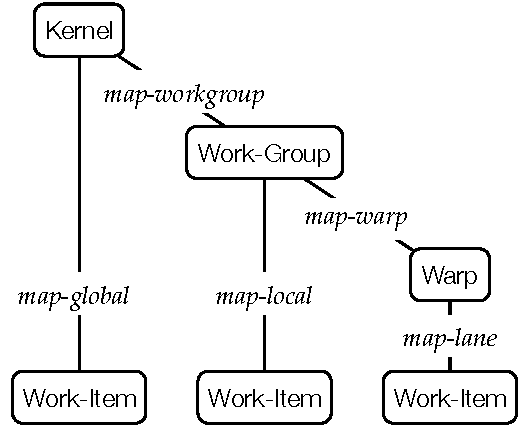
\includegraphics[width=.65\textwidth]{Figures/ThreadHierarchy.pdf}
  \caption{The \OpenCL thread hierarchy and the corresponding parallel \map patterns.}
  \label{fig:openclThreads}
\end{figure}
\autoref{fig:openclThreads} shows the \OpenCL thread hierarchy together with the corresponding parallel \map patterns:

\begin{itemize}
  \item The \mapGlobal pattern assigns work to work-items independent of their work-group, as shown on the left in \autoref{fig:openclThreads}.
        Following the definition of \map, each \OpenCL work-item executes its customizing function on a different part of the input array.

  \item The \mapWorkgroup pattern assigns work to an \OpenCL work-group and the \mapLocal pattern assigns work to a local work-item inside a work-group.
        This is shown in the middle of \autoref{fig:openclThreads}.
        The \mapLocal pattern only makes sense in the context of a work-group and is, therefore, only correctly used when nested inside a \mapWorkgroup pattern, \eg, $\mapWorkgroup\ (\mapLocal\ f)$.

  \item There are two additional patterns which are only valid when generating code for Nvidia \GPUs:
        \mapWarp and \mapLane.
        These are shown on the right of \autoref{fig:openclThreads}.
        These two patterns capture the notion of \emph{warps} present in Nvidia's \GPU architectures, \ie, 32 work-items are grouped and executed together (see \autoref{chapter:background} for details).
        Barrier synchronizations between work-items in the same warp can be avoided because a warp executes in a lock-step manner.
        To exploit this optimization we provide the \mapWarp pattern which assigns work to a warp, \ie, a group of 32 work-items.
        The \mapLane pattern is used to assign work to an individual work-item inside a warp.
\end{itemize}

%The code generation for all these map patterns is similar; we describe it using \pat{map-workgroup} as an example.
%A loop is generated, where the iteration variable is determined by the \emph{workgroup-id} function provided by \OpenCL.
%Inside of the loop, a pointer is generated to partition the input array, so that every work-group calls \pat{map-workgroup}'s customizing function on a different chunk of data.
%An output pointer is generated similarly.
%We continue with the body of the loop by generating the code for the customizing function recursively.
%Finally, an appropriate synchronization mechanism for the given map pattern is added.
%For instance after a \pat{map-local} we add a barrier synchronization to synchronize the threads inside of the work-group.

% \FloatBarrier

\paragraph{Sequential Map and Reduce}
The \mapSeq and \reduceSeq patterns perform a sequential map and reduction, respectively, within a single work-item.
% In both cases the generated code consists of a loop iterating over the array and calling the customizing function.
% For the reduction an accumulation variable is initialized with the given initial value and used to accumulate the results produced by the successive calls to to the customizing function.

For the \mapSeq pattern, the semantics and type are the same as for the high-level \map pattern shown in \autoref{definition:pattern:map}.
This is not the case for the \reduceSeq and \reduce patterns, where their types differ.
For the high-level \reduce pattern, we require the customizing binary operator to be associative and commutative in order to allow for an efficient parallel implementation.
As the \reduceSeq pattern performs a sequential reduction, we can relax these requirements, therefore, we define \reduceSeq separately.
\begin{definition}
  \label{definition:pattern:reduceSeq}
  Let $xs$ be an array of size $n$ with elements $x_i$ where $0 < i \leq n$.
  Let $\oplus$ be a binary customizing operator with the identity element $\id_\oplus$.
  The \reduceSeq pattern is then defined as follows:
  \begin{equation*}
    \reduceSeq\ (\oplus)\ \id_\oplus\ [x_1, x_2, \dots, x_n]
      \eqdef [(\dots((id_\oplus \oplus x_1) \oplus x_2) \ldots \oplus x_n)]
  \end{equation*}
  The types of $(\oplus)$, $\id_\oplus$, $\vec{x}$, and \reduce are as follows:
  \begin{align*}
    (\oplus) &: ((\alpha, \beta) \rightarrow \alpha),\\
    \id_\oplus &: \alpha,\\
    xs &: [\beta]_n,\\
    \reduceSeq\ (\oplus)\ \id_\oplus\ xs &: [\alpha]_1 .
  \end{align*}
\end{definition}


\paragraph{Reorder-stride}
The \reorderStride pattern enforces a special reordering of an array.
In our code generator (see \autoref{section:opencl:code:generator}) no code is produced for this pattern, but instead it affects how the following patterns reads it input from memory.
This pattern, therefore, indirectly produces a strided-access pattern which ensures that when each work-item accesses multiple elements two consecutive work-items access consecutive memory elements at the same time.
This corresponds to the \emph{coalesced memory accesses}, which are beneficial on modern \GPUs as discussed in \autoref{chapter:background}.
\begin{definition}
  \label{definition:pattern:reorderStride}
  Let $s$ be an integer value.
  Let $xs$ be an array of size $m$ with elements $x_i$, where $0 < i \leq m$.
  Let us assume that $m$ is evenly divisible by $s$ and that $m = s\times n$ for some integer value $n$.
  The \reorderStride pattern is then defined as follows:
  \begin{align*}
    \reorderStride\ s\ [x_1, x_2, \dots, x_m] &\eqdef [y_1, y_2, \dots, y_m], \text{ where}\\
    y_i &\eqdef x_{((i-1)\ \text{\normalfont div } n + s \times ((i-1) \bmod{n}))+1}
  \end{align*}
  Where $\text{\normalfont div}$ is integer division and $\bmod{}$ is the modulo operation.
  The types of $s$, $xs$, and \reorderStride are as follows:
  \begin{align*}
    s &: int,\\
    xs &: [\alpha]_m,\\
    \reorderStride\ s\ xs &: [\alpha]_m .
  \end{align*}
\end{definition}

\begin{figure}
  \centering
  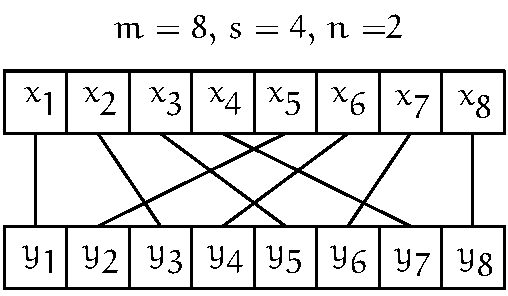
\includegraphics[width=0.5\textwidth]{Figures/Reorder.pdf}
  \caption[Visualization of the \reorderStride pattern]{Visualization of the \reorderStride pattern for an array of size 8 and a stride of 4}
  \label{fig:reorderStride}
\end{figure}
\autoref{fig:reorderStride} visualizes the reordering for an array $xs$ with 8 elements and a stride of 4.
In the reordered array the first two elements $y_1$ and $y_2$ correspond to $x_1$ and $x_5$.

% Our code generator produces no code directly, but rather the reordering determines how the data is read from the array in the following pattern.

%\noindent

%Our implementation does not produce code directly, but generates instead an index function, which is used when accessing the array the next time.
%Therefore, any following read implicitly reorders the array.
%Our design is general enough to supports user-defined index functions as well, which we will add in the future.
%The type of \pat{reorder-stride} corresponds to the type of the high-level \pat{reorder} pattern.

\paragraph{{\footnotesize to}Local and {\footnotesize to}Global}
The \toLocal and \toGlobal patterns are used to specify where the result of a given function $f$ should be stored.
As explained in more detail in \autoref{chapter:background}, \OpenCL defines two distinct address spaces: global and local.
Global memory is the commonly used large but slow memory.
On \GPUs, the comparatively small local memory has a high bandwidth with low latency and is used to store frequently accessed data.
With these two patterns, we can exploit the memory hierarchy defined in \OpenCL.

First, we define \toLocal:
\begin{definition}
  \label{definition:pattern:toLocal}
  Let $f$ be a function.
  The \toLocal pattern is then defined as follows:
  \begin{align*}
    \toLocal\ f &\eqdef f',
    \begin{aligned}[t]
      &\text{ where $f'\ x \eqdef f\ x$, $\forall x$, and  $f'$ is guaranteed to store}\\
      &\text{its result in local memory.}
    \end{aligned}
  \end{align*}
  The types of $f$, and \toLocal are as follows:
  \begin{align*}
    f &: (\alpha \rightarrow \beta),\\
    \toLocal\ f &: (\alpha \rightarrow \beta) .
  \end{align*}
\end{definition}

\noindent
The definition of \toGlobal is correspondent:
\begin{definition}
  \label{definition:pattern:toGlobal}
  Let $f$ be a function.
  The \toGlobal pattern is then defined as follows:
  \begin{align*}
    \toGlobal\ f &\eqdef f',
    \begin{aligned}[t]
      &\text{ where $f'\ x \eqdef f\ x$, $\forall x$ and $f'$ is guaranteed to store}\\
      &\text{ its result in global memory.}
    \end{aligned}
  \end{align*}
  The types of $f$, and \toGlobal are as follows:
  \begin{align*}
    f &: (\alpha \rightarrow \beta),\\
    \toGlobal\ f &: (\alpha \rightarrow \beta) .
  \end{align*}
\end{definition}

% These patterns act similarly to a typecast and are in fact implemented as such so that no code is emitted directly.

%In our design, every function reads its input and writes its output using pointers provided by the callee function.
%As a result, we can simply force a store to local memory by wrapping any function with our \pat{toLocal} pattern.
%In the code generator, this will simply change the output pointer of function $f$ to an area in local memory.

%The types of \pat{toLocal} and \pat{toGlobal} are identical and as follows:
%\begin{align}
%  f : (\alpha \rightarrow \beta)\ &\vdash\ toLocal\ f : (\alpha \rightarrow \beta)
%  \label{eq:type:toLocal}
%  \\
%  f : (\alpha \rightarrow \beta)\ &\vdash\ toGlobal\ f : (\alpha \rightarrow \beta)
%  \label{eq:type:toGlobal}
%\end{align}


\paragraph{{\footnotesize as}Vector, {\footnotesize as}Scalar, and Vectorize}
The \OpenCL programming model supports vector data types such as \code{float4} where operations on this type will be executed in the hardware vector units.
In the absence of vector units in the hardware, the \OpenCL compiler generates automatically a version of the code using scalar data types.

The \asVector and \asScalar patterns change the data type into vector elements and scalar elements, correspondingly.
For instance, an array of \code{float} is transformed into an array of \code{float4} as seen in the motivation example (\autoref{fig:codeex}).
%The \vect pattern vectorizes simple functions by converting all the operations that apply to vector types into vectorized operations.
%External tools~\cite{KarrenbergHa2011} have been developed for vectorizing more complex functions.
%Our current implementation can only vectorize functions containing simple arithmetic operations such as $+$ or $-$.
%These tools are not required to performing further analysis to find opportunities for vectorization.
%The rewrite rules presented in \autoref{section:rules} ensure that vectorization is only applied to patterns where vectorization is a legal optimization.

\bigskip

We start by defining the \asVector pattern.
\begin{definition}
  \label{definition:pattern:asVector}
  Let $n$ be a positive integer value.
  Let $xs$ be an array of size $m$ with elements $x_i$ where $0 < i \leq m$.
  Let us assume, that $m$ is evenly divisible by $n$.
  The \asVector pattern is then defined as follows:
  \begin{align*}
    &\asVector\ n\ [x_1, x_2, \dots, x_m] \eqdef \\
    &\qquad\big[\{x_1, \ldots, x_n\}, \{x_{n+1}, \ldots, x_{2n}\}, \ldots, \{x_{m-n+1}, \ldots, x_m\}\big],
  \end{align*}
  where $\{x_1,\ldots,x_n\}$ denotes a vector of width $n$.\\
  The types of $n$, $xs$, and \asVector are as follows:
  \begin{align*}
    n &: int\\
    xs &: [\alpha]_m,\\
    \asVector\ n\ xs &: [\alpha_n]_{\frac{m}{n}} .
  \end{align*}
  Here $\alpha$ is required to be a basic scalar type, \eg, \code{int} or \code{float}, and $\alpha_n$ denotes the vectorized version of that type with a vector width of $n$.
\end{definition}

\noindent
The corresponding \asScalar pattern is defined as follows.
\begin{definition}
  \label{definition:pattern:asScalar}
  Let $xs$ be an array of size $\frac{m}{n}$ whose elements are vectors of width $n$.
  We denote the individual vector elements of the $i$th element of $xs$ as $x_{((i-1)\times n)+j}$ where $0 < i \leq \frac{m}{n}$ and $0 < j \leq n$.
  The \asScalar pattern is then defined as follows:
  \begin{align*}
    &\asScalar_n\ \big[\{x_1, \ldots, x_n\}, \{x_{n+1}, \ldots, x_{2n}\}, \ldots, \{x_{m-n+1}, \ldots, x_m\}\big] \\
    & \qquad \eqdef [x_1, x_2, \dots, x_m],
  \end{align*}
  where $\{x_1,\ldots,x_n\}$ denotes a vector of width $n$.\\
  The types of $xs$, and $\asScalar_n$ are as follows:
  \begin{align*}
    xs &: [\alpha_n]_{\frac{m}{n}},\\
    \asScalar_n\ xs &: [\alpha]_m .
  \end{align*}
  Here $\alpha$ is required to be a basic scalar type, \eg, \code{int} or \code{float}, and $\alpha_n$ denotes the vectorized version of that type with a vector width of $n$.
\end{definition}

We will almost always omit the subscript for $\asScalar_n$, as $n$ can be inferred from the input array.

\bigskip

Finally, we define the \vect pattern.
\begin{definition}
  \label{definition:pattern:vect}
  Let $n$ be a positive integer value.
  Let $f$ be a function.
  The \vect pattern is then defined as follows:
  \begin{align*}
    \vect\ n\ f &\eqdef f_n, \text{ where } f_n\ \{x_1, \ldots, x_n\} = \{f\ x_1, \ldots, f\ x_n \}
  \end{align*}
  and $\{x_1,\ldots,x_n\}$ denotes a vector of width $n$.\\
  The types of $n$, $f$, and \vect are as follows:
  \begin{align*}
    n &: int,\\
    f &: (\alpha \rightarrow \beta),\\
    \vect\ n\ f &: (\alpha_n \rightarrow \beta_n) .
  \end{align*}
  Here $\alpha$ and $\beta$ are required to be basic scalar types, \eg, \code{int} or \code{float}, $\alpha_n$ and $\beta_n$ denote vectorized versions of these types with a vector width of $n$.
\end{definition}

\subsection{Summary}
In this section we introduced two type of \emph{patterns}:
high-level algorithmic patterns and low-level, \OpenCL-specific patterns.
While all of these patterns can be used by the application programmer to describe the solution for a particular problem, we expect the programmer to focus on the algorithmic patterns which should be used to express a high-level algorithmic implementation of the problem solution.
We will see in the next section how such an implementation composed of our high-level algorithmic patterns can be systematically rewritten using \emph{rewrite rules}.
During this process the original implementation will be modified and \OpenCL-specific patterns will be used.


